\capitulo{6}{Resultados}

\section{Resumen de resultados}

Se presenta en este capítulo un resumen de los resultados obtenidos durante el desarrollo del proyecto. 
\begin{itemize}
    
    \item \textbf{Elección de un sensor capaz de medir la fuerza ejercida por cada dedo.}
    
    Se ha utilizado el sensor de fuerza resistivo MD30-60, ofreciendo resultados satisfactorios en las pruebas realizadas. Con el objetivo de lograr un ajuste de las medidas lo más cercano a la realidad, se realizó una calibración en los sensores, para más detalle véase el Apendice G.1 del anexo. Además se realizó un análisis del porcentaje de error, ofreciendo como resultado, un valor de error medio de 4.6\%, con valores de pico de hasta un 10\% error.
    
    \item \textbf{Creación de un prototipo de dispositivo que pueda medir la presión ejercida por la mano.}
    
    Se ha logrado la creación de un prototipo funcional del dispositivo (\ref{fig:Prototipo Fisico}), cumpliendo con el diseño inicial de medir la presión ejercida por cada dedo de la mano de forma orientativa y repetible. Este prototipo integra cinco sensores de fuerza resistivos, una placa de arduino, una placa de pruebas, una luz led, un pin botón y otros materiales complementarios como resistencias y cables, proporcionando un prototipo integral que cumple con los requisitos necesarios. 

    Adicionalmente, se ha diseñado un accesorio complementario (\ref{fig:Accesorio}) que facilita el uso del dispositivo durante sesiones de rehabilitación. Tiene una dimensión de 60x60x135, con un agujero interior para insertar una de las barras de la
    tabla canadiense y cinco hendiduras destinadas a situar cada uno de los sensores.

    \begin{figure}
        \centering
        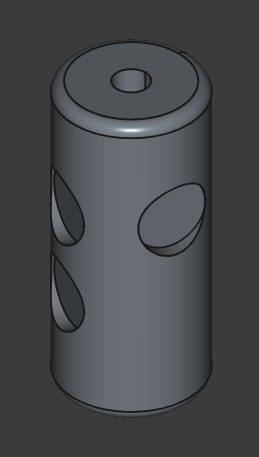
\includegraphics[width=0.25\linewidth]{img/Mango3.png}
        \caption{Accesorio para tabla canadiense. Fuente propia}
        \label{fig:Accesorio}
    \end{figure}
    \begin{figure}
        \centering
        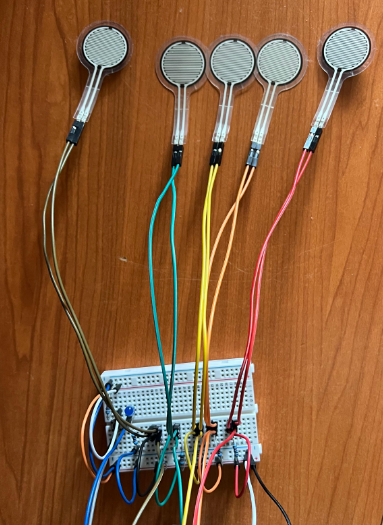
\includegraphics[angle=180,width=0.5\linewidth]{img/Prototipo_s.png}
        \caption{Prototipo físico. Fuente propia}
        \label{fig:Prototipo Fisico}
    \end{figure}
    \item \textbf{Seguimiento de evolución de los pacientes.}

    Se ha desarrollado un prototipo de interfaz tipo desplegable, capaz de almacenar los datos obtenidos por los sensores en un archivo xlsx. Además de su almacenamiento, permite al profesional la visualización de estos mediante una tabla (\ref{fig:tabla-registro}) o, representando los datos mediante una gráfica (\ref{fig:Grafica-datos}). 
    
    La estructura y visualización de los datos recolectados se amplía en el Apéndice D del anexo.
    \begin{figure}
        \centering
        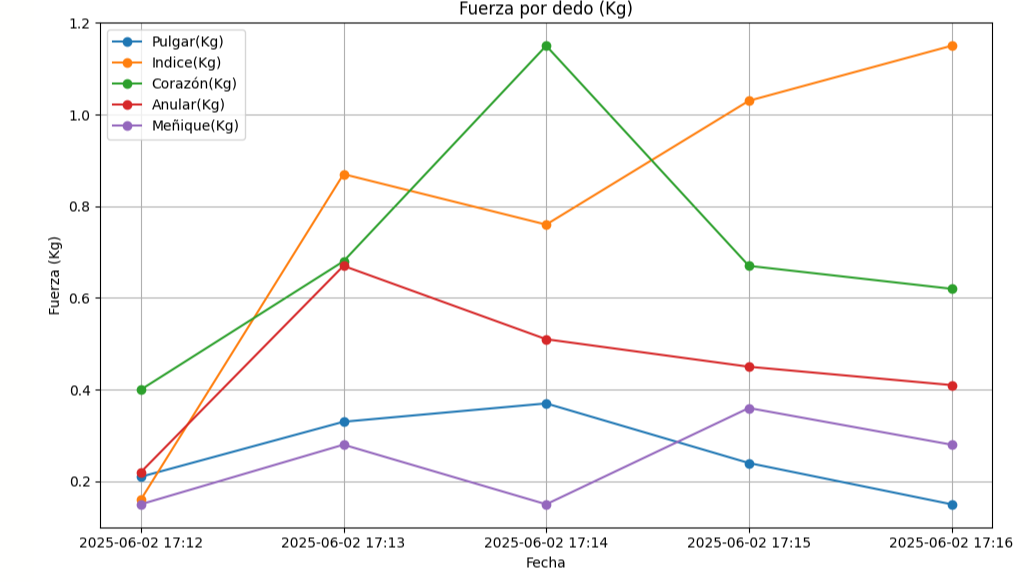
\includegraphics[width=0.8\linewidth]{img/grafica_fuerza.png}
        \caption{Representación datos en gráfica. Fuente propia}
        \label{fig:Grafica-datos}
    \end{figure}
    \begin{figure}
        \centering
        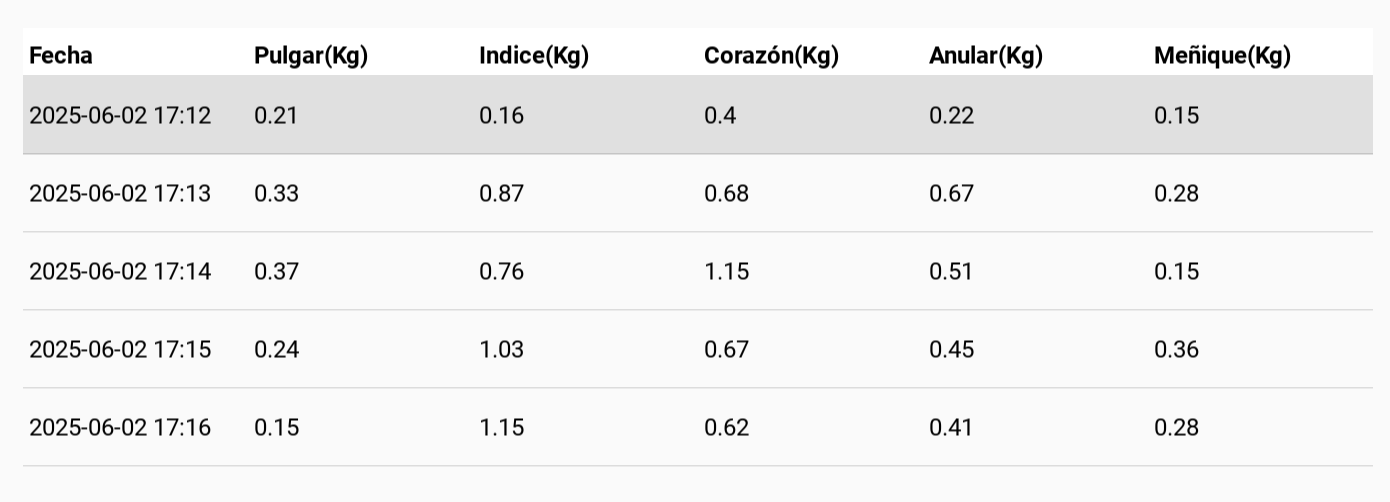
\includegraphics[width=1\linewidth]{img/Datos_medidas.png}
        \caption{Tabla de registros. Fuente propia}
        \label{fig:tabla-registro}
    \end{figure}
    \item \textbf{Comparativa de prototipos}
    
    Tras la realización del proyecto, he realizado una comparativa con otros prototipos mencionados en la sección 'Estado del arte'.

    A pesar de que los 3 prototipos emplean los sensores resistivos y tienen como finalidad el seguimiento de los pacientes para facilitar la recuperación, existen algunas diferencias. 
    En la tabla \ref{tab:comparacion_diseños} se presenta una comparativa de los 3 dispositivos.
\end{itemize}


\begin{table}[h]
    \centering
    \begin{tabular}{|p{2.5cm}|p{3.5cm}|p{4cm}|p{3.8cm}|}
    \rowcolor[HTML]{BFBFBF} 
    \hline
    \textbf{Aspecto} & \textbf{Juliana Gómez et al.} & \textbf{Luis Carlos Ralón Gordill} & \textbf{Diseño propio} \\ \hline
    Sensor utilizado   & FSR  & FSR  & FSR \\ \hline
    Número de sensores   & 5  & 1  & 5 \\ \hline
    Uso del resorte & Transmisión de fuerza & Generar resistencia  & No aplica   \\ \hline
    Mecanismo de transmisión   & Mediante resorte  & Mediante resorte & Directo  \\ \hline
    Ventajas   & Alta precisión  & Uso en niños  & Uso aplicabilidad múltiple \\ \hline
    Limitaciones & Solo permite el agarre de precisión & Fallos en Resorte-Sensor & Error medio de 4.6\% \\ \hline
    Visualización & Interfaz, visualización en el momento & Interfaz gráfica, visualización en el momento& Interfaz desplegable, con posibilidad de ver registros anteriores \\ \hline
    Coste    & No menciona    & No menciona precio exacto, pero deja claro que busca producir el menos coste y al utilizar un único sensor el coste total es bajo. & 78€ \\ \hline
    \end{tabular}
    \caption{Comparación de los prototipos.}
    \label{tab:comparacion_diseños}
\end{table}
    
\section{Discusión}

Los resultados obtenidos cumplen con los objetivos marcados en el inicio del proyecto. Se ha logrado realizar un prototipo de interfaz y dispositivo capaz de registrar los datos recogidos por los sensores.

La implementación de los gráficos en la visualización de los registros permite una representación clara de la evolución de los pacientes durante las sesiones. Facilitando la interpretación de los datos recogidos por los profesionales sanitarios, detectando progresos, fatiga muscular o estancamientos, factores muy útiles en la toma de decisiones médicas.

Además, la protección de los datos es uno de los aspectos fundamentales en la creación del dispositivo. Se cumplen en todo momento mediante la encriptación de los documentos. El uso de bibliotecas para el cifrado se detalla en el Apéndice C.1 y D.1 del anexo.

Por último, destacar la utilización de materiales que impliquen el menor coste posible en la realización del dispositivo. El análisis económico detallado y la viabilidad legal se exponen en los Apéndices A.3 y A.4 del anexo.